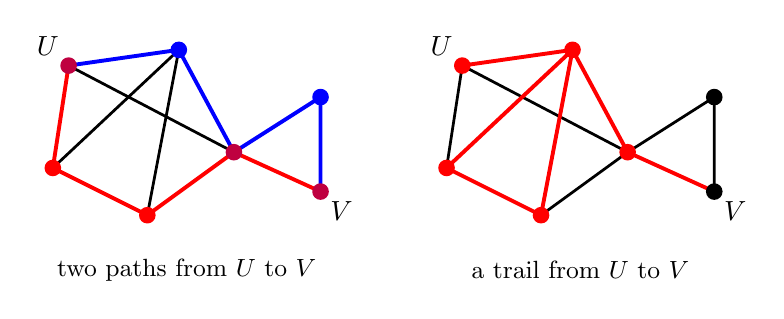
\begin{tikzpicture}[
  dot/.style={circle, fill, minimum size=6pt, inner sep=0pt},
  eb/.style={blue, line width=1.4pt},
  er/.style={red, line width=1.4pt},
  ek/.style={black, line width=1pt}]
% left: two paths from U to V (blue U-T-M-R-V, red U-L-B-M-V)
\begin{scope}
  \coordinate (U) at (0.2,2.0); \coordinate (T) at (1.6,2.2); \coordinate (M) at (2.3,0.9);
  \coordinate (R) at (3.4,1.6); \coordinate (V) at (3.4,0.4); \coordinate (L) at (0,0.7);
  \coordinate (B) at (1.2,0.1);
  \draw[ek] (U) -- (M); \draw[ek] (T) -- (L); \draw[ek] (T) -- (B);
  \draw[eb] (U) -- (T) -- (M) -- (R) -- (V);
  \draw[er] (U) -- (L) -- (B) -- (M) -- (V);
  \foreach \z in {U,M,V} \node[dot, purple] at (\z) {};
  \foreach \z in {T,R} \node[dot, blue] at (\z) {};
  \foreach \z in {L,B} \node[dot, red] at (\z) {};
  \node[above left] at (U) {$U$}; \node[below right] at (V) {$V$};
  \node[font=\small] at (1.7,-0.6) {two paths from $U$ to $V$};
\end{scope}
% right: a trail from U to V (U-T-L-B-T-M-V), revisiting the vertex T
\begin{scope}[xshift=5cm]
  \coordinate (U) at (0.2,2.0); \coordinate (T) at (1.6,2.2); \coordinate (M) at (2.3,0.9);
  \coordinate (R) at (3.4,1.6); \coordinate (V) at (3.4,0.4); \coordinate (L) at (0,0.7);
  \coordinate (B) at (1.2,0.1);
  \draw[ek] (U) -- (L); \draw[ek] (U) -- (M); \draw[ek] (B) -- (M); \draw[ek] (M) -- (R) -- (V);
  \draw[er] (U) -- (T) -- (L) -- (B) -- (T) -- (M) -- (V);
  \foreach \z in {U,T,L,B,M} \node[dot, red] at (\z) {};
  \foreach \z in {R,V} \node[dot, black] at (\z) {};
  \node[above left] at (U) {$U$}; \node[below right] at (V) {$V$};
  \node[font=\small] at (1.7,-0.6) {a trail from $U$ to $V$};
\end{scope}
\end{tikzpicture}
